% Chapter 4

\chapter{Methodology} % Main chapter title

\label{Chapter4} % For referencing the chapter elsewhere, use \ref{Chapter4} 

In this chapter, we present the methodology of the research. First we present
the threat model in section \ref{sec:threat-model}.  After that, we show the
overview of ScaRR algorithm to extract checkpoint and list of action in section
\ref{sec:overview}. Section \ref{sec:scarr-checkpoint-marker} discusses the LLVM
implementation to get checkpoints. Section \ref{sec:scarr-loa-collector}
discusses on methodology of getting list of actions.  
Checkpoints and list of actions are collected to build offline measurement 
database that is used for the remote attestation. The last section shows how to run the LLVM passes to 
get the result which is presented in Chapter \ref{Chapter5}.

\section{Threat Model}
\label{sec:threat-model}

The threat model in this research is taken from ScaRR
\cite{toffaliniScaRRScalableRuntime2019}. There are two parties: attacker and
prover. 

\vspace{0.5cm}
\noindent \textbf{Attacker capabilities:} The attacker aims to control remote
service using various method such as memory attack or any attack in user-space.
The attacker has bypassed memory attack protection such as Control Flow
Integrity (CFI) or \( W \bigoplus R \) or ASLR using techniques like
Return-Oriented Programming
(ROP)\cite{roemerReturnorientedProgrammingSystems2012} or Jump-Oriented
Programming (JOP) \cite{bletschJumpOrientedProgrammingNew2011}. We do not
consider physical attack and also non-control data attack which does not alter
program's CFG.

\vspace{0.5cm}
\noindent \textbf{Defender capabilities:} The prover uses kernel as trusted
anchor and has common memory corruption attack mitigations such as \( W
\bigoplus R \) and ASLR.  

\section{Overview of The Offline Measurement}\
\label{sec:overview}

\begin{figure}[htbp]
\centerline{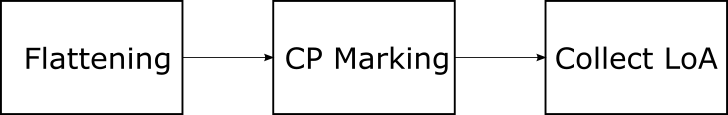
\includegraphics[scale=.75]{Figures/04/scarr-overview.png}}
\caption{Generating Offline Measurement}
\label{fig:scarr-overview}
\end{figure}

The goal of the offline measurement is to get the information to be used in the
remote attestation. In this research we implement ScaRR Control-flow model
\cite{toffaliniScaRRScalableRuntime2019} which we also elaborate in the Section
\ref{sec:scarr-model}. Figure \ref{fig:scarr-overview} shows the step on
generating the offline measurement.

We start with flattening the CFG into basic block. The CFG is structured as
graph that can contains branches and cycles. The flattening process will
traverse each and every graph once into a list of basic block. 

Consider the program in listing \ref{listing:simple-loop}. The CFG is shown in
the figure \ref{fig:simple-loop-cfg}. The first step of the offline measurement
is to flatten the CFG to get all the basic block list. We can flatten the CFG
into basic block with one out of some graph traversal algorithm in LLVM. The
result of flattened graph is in the right side of figure
\ref{fig:simple-loop-cfg}

\begin{listing}[htbp]
    \begin{minted}[
        frame=lines,
        framesep=2mm,
        baselinestretch=1.2,
        fontsize=\footnotesize
        ]{c++}
        int main() {
            for (int i = 0; i < 10; i++) {
                // do nothing
            }
        }
    \end{minted}
    \caption{Simple Loop}    
    \label{listing:simple-loop}
\end{listing}

\begin{figure}[htbp]
\centerline{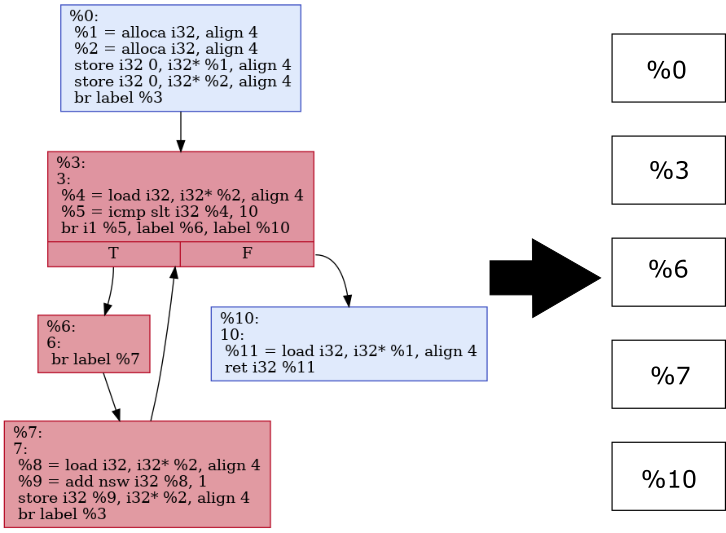
\includegraphics[scale=.70]{Figures/04/flatten-cfg.png}}
\caption{Simple Loop CFG}
\label{fig:simple-loop-cfg}
\end{figure}

After flattening the CFG we will have to pass the CFG for two times. First, to
mark the checkpoints (section \ref{sec:scarr-checkpoint-marker}). Second, to
find all list of actions between the checkpoint (section
\ref{sec:scarr-loa-collector}).

Checkpoints and list of actions are used to for offline measurements which is
represented as triplet of first and second checkpoint; and hash of the list of
actions.

$$(cp_A, cp_B, H(LoA)) \Rightarrow [(BBL_{s1}, BBL_{d1}), ..., (BBL_{sn},
BBL_{dn})]$$

The offline measurement is consulted by verifier during remote attestation.

\section{ScaRR Checkpoint Marker} 
\label{sec:scarr-checkpoint-marker}

After we flatten CFG into basic block, we will check each of basic block to find
different kind of checkpoints. In Chapter \ref{Chapter3} we list these four
types of checkpoints: \textbf{Thread Begin}, \textbf{Thread End}, \textbf{Exit
Point} and \textbf{Virtual Checkpoint}. Now we will present the heuristic on how
we will mark as a checkpoint when appropriate.  The logic of checkpoint marker
is to traverse the whole control flow graph at least once. For each basic block,
we have to check whether the basic block can be considered as any of checkpoint
type mentioned above. To allow marking additional information about ScaRR
checkpoint, we are modifying the BasicBlock class to add checkpoint instance
variable as shown in listing \ref{listing:checkpoint}.

\begin{listing}[htbp]
    \begin{minted}[
        frame=lines,
        framesep=2mm,
        baselinestretch=1.2,
        fontsize=\footnotesize,
        linenos
    ]{c++}
        class BasicBlock ... {
        private:
        // add checkpoint field
            Checkpoint cp;

        public:
            // setter and accessor
        void setCheckpoint(Checkpoint);
        Checkpoint getCheckpoint() const;
        ...
        }
    \end{minted}
    \caption{Add Checkpoint Instance Variable to BasicBlock class.}    
    \label{listing:checkpoint}
\end{listing}

Thread begin identifies the beginning of a thread or start of program. In this
thesis we mark this checkpoint to first basic block in main function. If a
program is is a multithreaded program, we will mark the thread begin for each
basic block that starts the thread.

In the other side, thread end marks the end of a thread or end of program. In a
multiple-threaded program, we will mark the thread end for each of basic block
that terminates a thread. In this thesis, we mark thread end checkpoint for last
basic block that has no more successors.

Exit point marks that a basic block is calling function outside of translation
unit. The heuristic of marking this type of basic block is we iterate all
instructions in a basic block. For each instruction, if the instruction is a
\texttt{call} instruction, we check whether the called function has any basic
block. If the function has no basic block, it means it is an external function,
hence we will mark this as an exit point and stop. If none of instruction is a
\texttt{call} instruction or all \texttt{call} instruction in this basic block
call function with non empty basic block, it means this basic block calls
internal function, therefore this basic block is not an exit point. Please refer
to Listing \ref{listing:exit-point-cp}.

\begin{listing}[htbp]
    \begin{minted}[
        frame=lines,
        framesep=2mm,
        baselinestretch=1.2,
        fontsize=\footnotesize,
        linenos
    ]{c++}
        for (auto &basicBlock: Function) {
            for (auto &instruction : basicBlock) {
                if (isa<CallInst>(i)) {
                auto *call = &cast<CallBase>(i);
                if (call != nullptr && call->getCalledFunction()->empty()) {
                    // this basicBlock is ExitPoint
                    basicBlock.setCheckpoint(Checkpoint::ExitPoint);
                } 
            }
        } 
    \end{minted}
    \caption{Finding ExitPoint Checkpoint}    
    \label{listing:exit-point-cp}
\end{listing}

Virtual checkpoint is a checkpoint that marks special cases such as loop or
recursion. We will discuss only for loop case in this thesis. Virtual checkpoint
in a loop is basically a loop header. The heuristic to find a loop header is to
use \texttt{DominatorTree} to find a loop. After we find a loop, then we just
need to get the header. Although there is no direct API to check whether a basic
block is a loop header, LLVM provide it in LoopInfoBase API. See Listing
\ref{listing:virtual-cp}

\begin{listing}[htbp]
    \begin{minted}[
        frame=lines,
        framesep=2mm,
        baselinestretch=1.2,
        fontsize=\footnotesize,
        linenos
    ]{c++}
        void findVirtualCheckpoint(DominatorTree &DT, Function &F) {
            DT.recalculate(F);
            // generate the LoopInfoBase for the current function
            LoopInfoBase<BasicBlock, Loop>* KLoop = new LoopInfoBase<BasicBlock, Loop>();
            KLoop->releaseMemory();
            KLoop->analyze(DT);
            for (auto &bb : F) {
                // Since the BasicBlock would have been inlined, just traverse from main function
                if (F.getName() == "main") {
                auto loop = KLoop->getLoopFor(&bb);
                if (loop != nullptr) {
                    // found VirtualCheckpoint
                            loop->getHeader()->setCheckpoint(Checkpoint::Virtual);
                }
                }
            }
        }
    \end{minted}
    \caption{Getting Virtual Checkpoint}
    \label{listing:virtual-cp}
\end{listing}



\begin{figure}[htbp]
\centerline{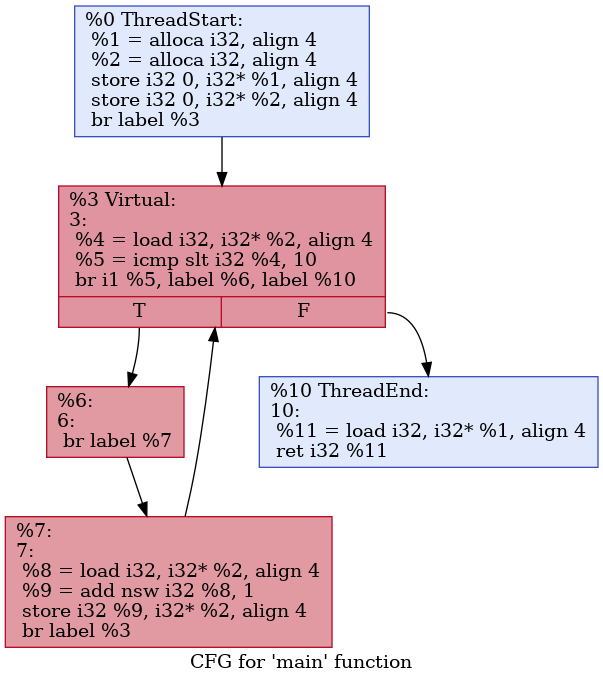
\includegraphics[scale=.70]{Figures/04/simple-loop-checkpoints.png}}
\caption{Loop CFG}
\label{fig:simple-loop-checkpoints}
\end{figure}

\section{ScaRR LoA Collector} \label{sec:scarr-loa-collector} After we mark
checkpoints in the CFG, now we can find list of actions. The step of finding LoA
is traversing path between two checkpoints and add significant basic block that
traverse the path between the two checkpoints. The detail of this step is
explained in section \ref{sec:scarr-loa-collector}.

\xt{TODO: summarize the algorithm in a pseudocude fashion? you should link the
lines in the pseudo code and describe it step by step.}

\begin{listing}[htbp]
    \begin{minted}[
        frame=lines,
        framesep=2mm,
        baselinestretch=1.2,
        fontsize=\footnotesize,
        linenos
    ]{c++}
    // TBD
    \end{minted}
    \caption{TBD Pseudocode for LoA}
    \label{listing:loa-pseudocode}
\end{listing}

The algorithm of getting LoA between two checkpoints is little bit more complex.
First, we iterate all the basic block and if the basic block is a checkpoint we
mark this is $cpA$. Next, we recursively traverse the successor of $cpA$ until
we find another checkpoint $cpB$. It is possible for $cpA = cpB$. If there is no
branch between the two checkpoint, the LoA is an empty set. If there is a
branch, the first LoA is always be $cpA$ and the second LoA is always be the
first basic block after the branch \textemdash{} which can be $cpB$ or just non
checkpoint basic block. Interested readers can refer to the implementation of
this pass to see the detail.

\section{Running The Pass}

To mark the list of Checkpoints, we can invoke LLVM \texttt{opt} as shown in
listing \ref{listing:mark-cp-in-cfg}.

\begin{listing}[htbp]
    \begin{minted}[
        frame=lines,
        framesep=2mm,
        baselinestretch=1.2,
        fontsize=\footnotesize,
    ]{c++}
        opt -passes=scarr-cp-marker <file>.ll
    \end{minted}
    \caption{Mark Checkpoint in BasicBlock}    
    \label{listing:mark-cp-in-cfg}
\end{listing}

We can see the basic blocks output that has been marked with checkpoint using
LLVM dot-cfg pass.

\begin{listing}[htbp]
    \begin{minted}[
        frame=lines,
        framesep=2mm,
        baselinestretch=1.2,
        fontsize=\footnotesize,
    ]{c++}
        opt -passes=scarr-cp-marker,dot-cfg <file>.ll
    \end{minted}
    \caption{Print Checkpoints in CFG dot file}    
    \label{listing:cp-to-cfg}
\end{listing}

The commands in listing \ref{listing:cp-to-cfg} generates different dot files
per function. We can use xdot command line from graphiz to see the graph. 

To mark the list of actions between checkpoints, we can invoke LLVM \texttt{opt}
as shown in Listing \ref{listing:get-loa}

\begin{listing}
    \begin{minted}[
        frame=lines,
        framesep=2mm,
        baselinestretch=1.2,
        fontsize=\footnotesize,
    ]{c++}
        opt -passes=scarr-cp-marker,scarr-loa-collector <file>.ll
    \end{minted}
    \caption{Get List of Actions}    
    \label{listing:get-loa}
\end{listing}

Note that we have to run scarr-cp-marker before scarr-loa-collector.

The result and its interpretation are discussed in the next chapter.